% Шаблон для оформления работ в ВШЭ
% Используется xelatex

\documentclass[a4paper,10pt]{article}

%%% Работа с русским языком
\usepackage[utf8]{inputenc}		% кодировка исходного текста
\usepackage[T2A]{fontenc}			% кодировка
\usepackage{cmap}					% поиск в PDF
\usepackage{mathtext} 				% русские буквы в формулах
\usepackage[english,russian]{babel}	% локализация и переносы

%%% Дополнительная работа с математикой
\usepackage{amsmath,amsfonts,amssymb,amsthm,mathtools} % AMS
\usepackage{icomma} % "Умная" запятая: $0,2$ --- число, $0, 2$ --- перечисление


%%% Рисунки
\usepackage[format=plain,
            font={small,it},
            figurename=Рисунок,
            figurewithin=section,
            labelsep=endash % Разделитель между числом и подписью (--)
            ]{caption}

%%% Заголовки
\usepackage{titlesec}
\renewcommand{\numberline}[1]{#1~}
\titleformat{\section}[block]{\fontsize{16}{12}\selectfont\bfseries\filcenter}{\thesection}{4pt}{}
\titleformat{\subsection}[block]{\fontsize{14}{12}\bfseries\filcenter}{\thesubsection}{4pt}{}
% \renewcommand{\thesection}{Глава \arabic{section} --}
% \renewcommand{\thesubsection}{\arabic{section}.\arabic{subsection} --}


\titlespacing*{\section}
{0pt}{0pt}{12pt} % left, top, bottom
\newcommand{\sectionbreak}{\clearpage}

\titlespacing*{\subsection}
{0pt}{12pt}{6pt}

%%% Оглавление
\usepackage{tocloft}
\renewcommand{\cftsecleader}{\cftdotfill{\cftdotsep}} % точки в оглавлении
\renewcommand\cfttoctitlefont{\hfill\Large\bfseries} % заголовок оглавления по центру
\renewcommand\cftaftertoctitle{\hfill\mbox{}} % продолжение заголовок по центру


%%% Работа с картинками
\usepackage{graphicx}  % Для вставки рисунков
\graphicspath{{diagrams/}{images/}{images2/}}  % папки с картинками
\setlength\fboxsep{3pt} % Отступ рамки \fbox{} от рисунка
\setlength\fboxrule{1pt} % Толщина линий рамки \fbox{}
\usepackage{wrapfig} % Обтекание рисунков текстом

%%% Работа с таблицами
\usepackage{array,tabularx,tabulary,booktabs} % Дополнительная работа с таблицами
\usepackage{longtable}  % Длинные таблицы
\usepackage{multirow} % Слияние строк в таблице

\newtheorem*{nonum}{Решение}

%%% Страница
\usepackage[fontsize=13pt]{scrextend}
\usepackage{geometry} % Простой способ задавать поля
	\geometry{top=20mm}
	\geometry{bottom=20mm}
	\geometry{left=30mm}
	\geometry{right=15mm}

\usepackage{setspace} % Интерлиньяж 1.5
    \onehalfspacing

\usepackage{indentfirst} % Абзацные отступы
    \setlength{\parindent}{1.25cm}


\usepackage[normalem]{ulem} % для подчёркиваний uline
    \ULdepth = 0.2em % расстояние от линии до текста выше/ниже


\usepackage{fontspec}
    \setmainfont{Times New Roman}


\begin{document} % конец преамбулы, начало документа

\thispagestyle{empty}
\begin{center}
    \begingroup
    \fontsize{13pt}{15pt}\selectfont

    Пермский филиал федерального государственного автономного \\
    образовательного учреждения высшего образования \\
    <<Национальный исследовательский университет \\
    <<Высшая школа экономики>>

	\vspace{2em}
    \textit{Факультет экономики, менеджмента и бизнес-информатики}

    \vspace{4em}
    Бочкарев Вадим Александрович

    \vspace{3em}
    % \textbf{ФОРМИРОВАНИЕ ТРЕБОВАНИЙ К ПРОГРАММНОЙ СИСТЕМЕ}
    \textbf{НАЗВАНИЕ ТЕМЫ КУРСОВОЙ РАБОТЫ}

    \vspace{0.5em}
    \textit{Отчёт по лабораторной работе}

    \vspace{3em}

\fontsize{13pt}{15pt}\selectfont
    студента образовательной программы бакалавриата <<Программная инженерия>>\\
    по направлению подготовки \textit{\uline{09.03.04 Программная инженерия}}

\vfill

\hfill % заполнить пустоту по ширине
\parbox{6cm}{

    \fontsize{13pt}{15pt}\selectfont
    \begin{flushleft}
            Руководитель\\
            преподаватель кафедры\\
            информационных технологий в бизнесе

            \hrulefill

            В.П. Куприн
    \end{flushleft}
}

\vfill

\endgroup
\center{Пермь, 2021}\end{center}\newpage


\tableofcontents
\clearpage

% \section{Введение}

% В данной работе проводится анализ поставленной задачи,
% формулирование требований к проектируемой системе,
% определяются основные варианты использования и ограничения.

% Рассматривается система <<Машина состояний>>.

\section{Анализ задачи}

\subsection{Описание решаемой задачи}

Машина состояний является сущностью, которая на основе
переданных настроек (описание жизненного цикла типа объектов, начальное состояние)
вычисляет текущее состояние объекта, изменяет его в зависимости от переданных данных
(некие события или же изменения в самих объектах).

Рассмотрим, что из собой представляют инициализирующие настройки машины состояний.
Описание жизненного цикла типа объектов заключается в наборе состояний машины и
правилах перехода между ними. Начальное состояние уже описывает конкретный объект;
оно содержит информацию о самом объекте (некий набор его характеристик) и текущее
состояние с точки зрения машины состояний.


\subsection{Диаграмма прецедентов}

Для построения диаграммы прецедентов необходимо выделить акторов, непосредственно
сами прецеденты и определить типы связей между ними.



\begin{figure}[htpb]
    \centering
    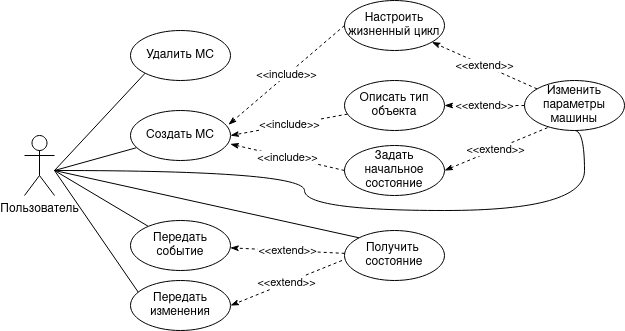
\includegraphics[width=0.8\textwidth]{Use Case}
    \caption{Use case диаграмма}
    \label{fig:useCase}
\end{figure}

В качестве актора проектируемой системы выступит абстрактный Пользователь.
Пользователь инициализирует машину состояний и взаимодействует с ней.

Инициализация происходит посредством передачи параметров жизненного цикла,
описания типа объектов и задания некоего начального состояния. Три вышеназванных
действия выступят в качестве прецедентов, которые будут включены в прецедент создания
и расширять прецедент редактирования.

Пользователь сможет передавать системе информацию о том, что происходит с объектом.
Это возможно двумя способами: передача информации о неком событии или же передача
непосредственно изменений объекта.

Пользователь должен иметь возможность в любой момент времени получить информацию
о текущем состоянии машины состояний, вынесем это в отдельный прецедент. Логично
предположить, что при передаче пользователем информации об изменениях целесообразно
добавить возможность получить сразу же новое состояние системы. Этот фактор необходимо
будет обозначить на диаграмме.

Наконец, пользователь должен иметь возможность удалить машину состояний.

Обозначим всё вышесказанное на диаграмме прецедентов (см. Рисунок \ref{fig:useCase}).

\subsection{Формирование требований}

Исходя из выделенных ранее прецедентов определим функциональные требования к
проектируемой системе:

\begin{itemize}
    \item Создать машину состояний;
    \item Изменить параметры машины состояний;
    \item Удалить машину состояний;
    \item Передать событие;
    \item Передать изменения.
\end{itemize}

Рассмотрим нефункциональные требования к системе.

Взаимодействие с машиной состояния должно быть максимально удобным для пользователя,
она должна максимально абстрагировать своё внутреннее устройство и предоставлять
простой и комфортный интерфейс взаимодействия.

В качестве следующего нефункционального требования рассмотрим устойчивость.
Система должна корректно обрабатывать непредвиденные ситуации, например,
давать информативные сообщения об ошибках. Ошибки могут быть связаны, к примеру,
с появлением события, не описанного в жизненном цикле.

Система должна быть эффективной: поскольку вполне возможно, что ей предстоит
взаимодействовать с большим числом объектов, а вычислительные ресурсы машин ограничены.



\end{document} % конец документа
